\section{Source Code and Data Sources}
\label{ch:codesource}

Much of the code was written from scratch for this project, or is a close to direct translation of the formulas described in papers such as Grigorian's \cite{grigor20}.

\subsection{R packages}

\verb|ggplot2|  \cite{ggplot2} is widely used for easily plotting and visualising the models. \verb|rgdal| \cite{rgdal} allows geospatial \verb|.shp| files to be read into \verb|R|. 

\verb|raster| \cite{raster} allows this data to be manipulated and plotted. 

\verb|dplyr| \cite{dplyr}  provides useful data manipulation functions, both for models and geospatial mapping. 

Statistical models (HoltWinters, ARIMA and Neural Network Regression) were readily implemented from \verb|forecast| \cite{forecast}.

The majority ofthe colours for plotting are selected using colour oalettes from the \verb|wesanderson| package \cite{wesanderson20}.

\begin{figure}[!htb]
\minipage{0.98\textwidth}
  
\includegraphics[width=\linewidth]{wespalette.png} \label{fig:wespalette}
  
\includegraphics[width=\linewidth]{wespalette2.png} \label{fig:wespalette2}
  
\includegraphics[width=\linewidth]{wespalette3.png} \label{fig:wespalette3}
\endminipage
\caption{Wes Anderson Palettes}
\end{figure}


\subsection{Shapefiles}

This data includes the geospatial vector data which can be used to \textit{draw} country (and county) coastlines and borders. 

World country shape data was obtained from \cite{countryshape}, while the more detailed county-level shapefile was downloaded from \cite{countyshape}.

\subsection{Datasets}

\underline{Country-based data:}

Originally used data from \cite{ecdcdata},  but the ECDC switched from a daily to a weekly update from 14 December 2020. Therefore, I have chosen to use the data from  \cite{countrydata}, which has remained daily

\begin{figure}[H]
\minipage{0.98\textwidth}
  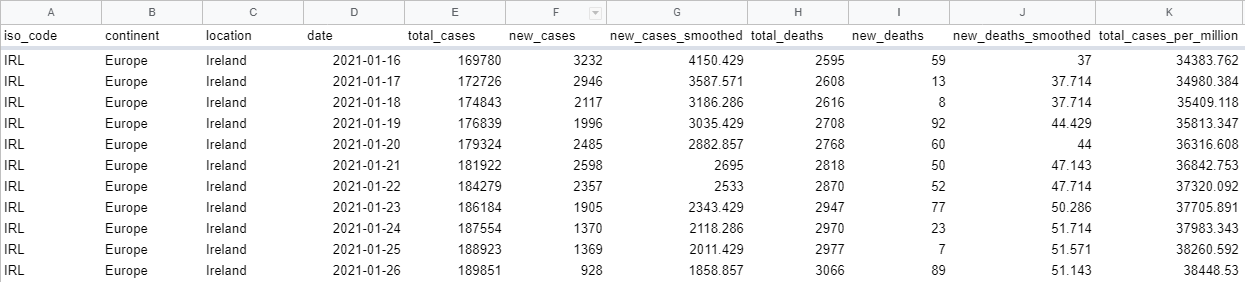
\includegraphics[width=\linewidth]{owiddatextract.png} \label{fig:owiddatextract}
\endminipage
\caption{OWID World data extract}
\end{figure}

\underline{Ireland cases by county}

Downloaded from \cite{irelanddata}.

\begin{figure}[H]
\minipage{0.98\textwidth}
  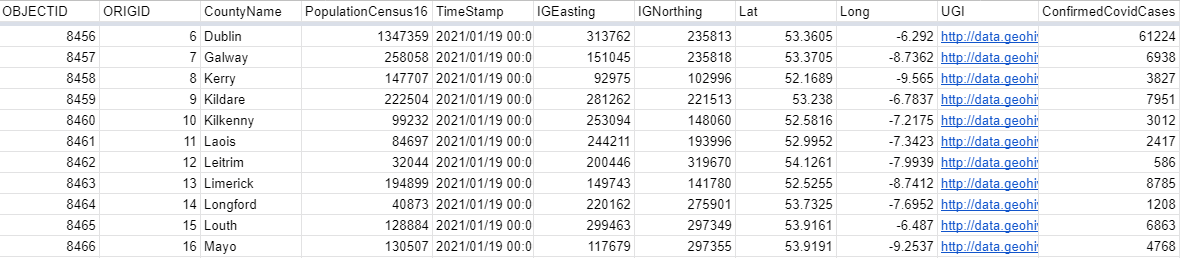
\includegraphics[width=\linewidth]{irelanddatextract.png} \label{fig:irelanddatextract}
\endminipage
\caption{ArcGIS Ireland data extract}
\end{figure}


\subsection{Source Code}

All the code, plots, and even this report, are available at \url{https://github.com/gibbona1/TCD_FinalYearProject}. 

I will include the main code files in text below.

\lstinputlisting[frame=single, caption = {Model helper functions}, label={lst:covidmodelutils}]{C:/Users/Anthony/Documents/GitHub/TCD_FinalYearProject/Code/covid-modelutils.R}

\lstinputlisting[frame=single, caption = {Plotting functions},  label={lst:covidplotutils}]{C:/Users/Anthony/Documents/GitHub/TCD_FinalYearProject/Code/covid-plotutils.R}

\lstinputlisting[frame=single, caption = {Main algorithm},  label={lst:covidmain}]{C:/Users/Anthony/Documents/GitHub/TCD_FinalYearProject/Code/covid-main.R}

\lstinputlisting[frame=single, caption = {multi-phase models},  label={lst:covidmultimodel}]{C:/Users/Anthony/Documents/GitHub/TCD_FinalYearProject/Code/covid-multimodel.R}

\lstinputlisting[frame=single, caption = {Geospatial/Map plots},  label={lst:covidmapplots}]{C:/Users/Anthony/Documents/GitHub/TCD_FinalYearProject/Code/covid-mapplots.R}

\lstinputlisting[frame=single, caption = {Country Comparison plots},  label={lst:covidcompare}]{C:/Users/Anthony/Documents/GitHub/TCD_FinalYearProject/Code/covid-compare.R}

\lstinputlisting[frame=single, caption = {Saving plots},  label={lst:saveplots}]{C:/Users/Anthony/Documents/GitHub/TCD_FinalYearProject/Code/saveplots.R}